\documentclass{article}
\usepackage{graphicx} % Required for inserting images
\usepackage{minted}
\newcommand{\pder}[2][]{\frac{\partial#1}{\partial#2}}
\newcommand{\sder}[2][]{\frac{\partial^2#1}{\partial#2^2}}

\title{Computational Physics}
\author{Alex Zhou}
\date{May 2019}

\begin{document}

\maketitle

\section{The Restricted Three Body Problem}

For two bodies, there is a stable analytic solution which describes the rotation around a joint centre of mass. For three bodies, in general the solution cannot be obtained analytically. For this reason, we consider the restricted problem where the third body has negligible mass and therefore does not affect the other two's motion. The problem is to solve for the motion of the third body under the gravitational influence of the other two.

Transform the frame of reference such that the first two bodies appear stationary and the origin corresponds to their joint centre of mass. Scale the space so that the angular velocity in this frame is \(1\) and the distance between the two bodies is \(1\). The only parameter \(\mu\) is the quantity defined such that the two masses are in the ratio \(\mu : 1 - \mu\), and are situated at the two points \(P_1 = (\mu - 1, 0)\) and \(P_2 = (\mu, 0)\). At time \(t\), the third body has position \((x(t), y(t))\) and its equation of motion is the ordinary differential equation
\[ \ddot{x} - 2\dot{y} = -\pder[\Omega]{x}, \quad \ddot{y} + 2\dot{x} = -\pder[\Omega]{y}, \]
where the potential is defined by
\[ \Omega = -\frac{1}{2}\mu r_1^2 \frac{1}{2}(1-\mu)r_2^2 - \frac{\mu_1}{r_1} - \frac{1-\mu}{r_2}, \]
with \(r_1^2 = (x+1-\mu)^2 + y^2\) and \(r_2^2 = (x-\mu)^2 + y^2\). Despite this restriction of the full three body problem, it is still not possible to solve this analytically.

Consider the Jacobi quantity given by the sum of the kinetic energy and potential energy
\[ J = \frac{1}{2}\dot{x} + \frac{1}{2}\dot{y} + \Omega(x, y). \]
Then by differentiating once
\[ \dot{J} = \dot{x}\ddot{x} + \dot{y}\ddot{y} + \pder[\Omega]{x}\dot{x} + \pder[\Omega]{y}\dot{y} = \dot{x}\left(2\dot{y} -\pder[\Omega]{x}\right) + \dot{y}\left(-2\dot{x} -\pder[\Omega]{y}\right) + \pder[\Omega]{x}\dot{x} + \pder[\Omega]{y}\dot{y} = 0. \]
Hence \(J\) is constant. Let \(x_0\) and \(y_0\) be the initial values and \(u_0\) and \(v_0\) be the initial velocities. Then
\[ J = \frac{1}{2}u_0^2 + \frac{1}{2}v_0^2 + \Omega(x_0, y_0), \]
where the first two terms are non-negative, so
\[ \Omega(x, y) = J - \frac{1}{2}\dot{x }+ \frac{1}{2}\dot{y} \leq J = \frac{1}{2}u_0^2 + \frac{1}{2}v_0^2 + \Omega(x_0, y_0). \]
This shows that the trajectories must be confined to the region where \(\Omega(x,y)\) is less than or equal to the (initial) value of \(J\).

We shall implement a numerical ODE solver for the restricted three body problem. To do this, we will convert the system of two second order ordinary differential equations to a system of four first order ordinary differential equations. We first directly compute the partial derivative of the \(r_1, r_2, \Omega\),
\[ \pder[r_1]{x} = \frac{x+1 - \mu}{r_1}, \quad \pder[r_1]{y} = \frac{y}{r_1}, \quad \pder[r_2]{x} = \frac{x-\mu}{r_2}, \quad \pder[r_2]{y} = \frac{y}{r_2}. \]
Hence
\begin{eqnarray*}
    \pder[\Omega]{x} & = & -\mu r_1\pder[r_1]{x} - (1-\mu)r_2\pder[r_2]{x} + \frac{\mu}{r_1^2}\pder[r_1]{x} + \frac{1-\mu}{r_2^2}\pder[r_2]{x} \\
                     & = & -\mu(x+1-\mu) - (1-\mu)(x-\mu) + \frac{\mu(x+1-\mu)}{r_1^3} + \frac{(1-\mu)(x-\mu)}{r_2^3} \\
                     & = & -x + \frac{\mu(x+1-\mu)}{r_1^3} + \frac{(1-\mu)(x-\mu)}{r_2^3}.\\
    \pder[\Omega]{y} & = & -\mu r_1\pder[r_1]{y} - (1-\mu)r_2\pder[r_2]{y} + \frac{\mu}{r_1^2}\pder[r_1]{y} + \frac{1-\mu}{r_2^2}\pder[r_2]{y} \\
                     & = & -\mu y - (1-\mu)y + \frac{\mu y}{r_1^3} + \frac{(1-\mu)y}{r_2^3} \\
                     & = & -y + \frac{\mu y}{r_1^3} + \frac{(1-\mu)y}{r_2^3}.
\end{eqnarray*}

The following computes the potential \(\Omega\) and its derivatives at a single point:

\begin{minted}[autogobble, linenos]{Python}
    import numpy as np
    from scipy.integrate import solve_ivp
    import matplotlib.pyplot as plt
    
    def Omega_potential_and_derivatives(x, y, mu):
        # Positions and distances
        P1_x = mu - 1
        P2_x = mu
        r1_sq = (x - P1_x)**2 + y**2
        r2_sq = (x - P2_x)**2 + y**2
        r1 = np.sqrt(r1_sq)
        r2 = np.sqrt(r2_sq)
    
        Omega = - mu*r1_sq/2 - (1 - mu)*r2_sq/2 - mu/r1 - (1 - mu)/r2
        Omega_dx = -x + mu*(x - P1_x)/r1**3 + (1 - mu)*(x - P2_x)/r2**3
        Omega_dy = -y + mu * y/r1**3 + (1 - mu) * y/r2**3
        return Omega, Omega_dx, Omega_dy
\end{minted}

From here, we can use this to produce a contour plot of the potential. Furthermore, we can implement an ODE solver to compute a trajectory given a parameter \(\mu\), initial conditions and short time interval.

\begin{minted}[autogobble, linenos]{python}
    def three_body_ode_system(t, z, mu):
        x, y, x_dot, y_dot = z
        Omega_dx, Omega_dy = potential_and_derivatives(x, y, mu)
        x_ddot = 2 * y_dot - Omega_dx
        y_ddot = -2 * x_dot - Omega_dy
        return [x_dot, y_dot, x_ddot, y_ddot]
    
    def get_three_body_trajectory(mu, initial, t_span, num_points=10000):
        t_eval = np.linspace(t_span[0], t_span[1], num_points)
        solution = solve_ivp(
            fun=three_body_ode_system,
            t_span=t_span,
            y0=initial,
            args=(mu,),
            t_eval=t_eval,
            dense_output=True,
            rtol=1e-12,
            atol=1e-12
        )
        return solution.t, solution.y
\end{minted}

In order to verify that our numerical solution is accurate, we can use the Jacobi quantity \(J\) and verify that it is constant. We can achieve this by computing \(J\) on the trajectory, and plotting the change in \(J\) over time, relative to its initial value \((J(t) - J_0) / J_0\).

\begin{minted}[autogobble]{python}
    def calculate_jacobi_integral(state_vector, mu):
        x, y, x_dot, y_dot = state_vector
        kinetic_energy = (x_dot**2 + y_dot**2) / 2
        potential_energy = calculate_Omega_and_derivatives(x, y, mu)[0]
        return kinetic_energy + potential_energy
\end{minted}

\section{Space Travel}

Let us first assume that the first two bodies have equal mass so \(\mu = \frac{1}{2}\) and consider the motion of a 'spacecraft' near \(P_2\) so that the effect of \(P_1\) may be ignored and the potential can be approximated by
\[ \Omega = -\frac{1}{r_2}. \]
The equations of motion remain the same but now we change coordinates to the location of \(P_2 = (\mu, 0)\) via \(x' = x - \mu\) and \(y' = y\), where the derivatives all remain the same. In these new coordinates, the new distance to \(P_2\) is simply \(r_2^2 = x'^2 + y'^2\) therefore 
\[ \frac{\partial\Omega}{\partial x} = \frac{\partial\Omega}{\partial x'} = -\frac{1}{2} \left(-\frac{1}{2}\right) (x'^2 + y'^2)^{-3/2} (2x') = \frac{x'}{2r_2^3}, \]
and
\[ \frac{\partial\Omega}{\partial y} = \frac{\partial\Omega}{\partial y'} = -\frac{1}{2} \left(-\frac{1}{2}\right) (x'^2 + y'^2)^{-3/2} (2y') = \frac{y'}{2r_2^3}. \]
Substituting into the original equations of motion, we obtain
\[ \ddot{x'} - 2\dot{y'} = -\frac{x'}{2r_2^3}, \quad \ddot{y'} + 2\dot{x'} = -\frac{y'}{2r_2^3}. \]
We claim that some analytic solutions of this system are circular orbits about \(P_2\) of small positive radius \(a>0\) depending on the initial conditions. To see this, first we define the circular orbit ansatz with angular velocity \(\omega\) by
\[ x'(t) = a\cos(\omega t), \quad y'(t) = a\sin(\omega t), \]
which has first derivatives
\[ \dot{x'}(t) = -a\omega \sin(\omega t), \quad \dot{y'}(t) = a\omega \cos(\omega t) \]
and second derivatives
\[ \ddot{x'}(t) = -a\omega^2 \cos(\omega t), \quad \ddot{y'}(t) = -a\omega^2 \sin(\omega t). \]
Substituting into the first equation of motion gives
\[ -a\omega^2 \cos(\omega t) - 2a\omega \sin(\omega t) = -\frac{a\cos(\omega t)}{2a^3}, \]
which holds only if
\[ \omega^2 + 2\omega = \frac{1}{2a^3}. \]
Similarly, substituting into the second equation of motion gives
\[ -a\omega^2 \sin(\omega t) - 2a\omega \sin(\omega t) = -\frac{a\sin(\omega t)}{2a^3}, \]
which again holds only if
\[ \omega^2 + 2\omega = \frac{1}{2a^3}. \]
Solving the resulting quadratic equation yields two solution for the angular velocity
\[ \omega = -1 \pm \sqrt{1 + \frac{1}{2a^3}}, \]
which correspond to the prograde and retrograde orbits and is valid for any small \(a > 0\). Note that the period of the orbit is given by
\[ T = \frac{2\pi}{|\omega|}. \]
In our plot, we shall take the initial position to be on the right side of \(P_2\), so \(x'_0 = 0\) and \(y'_0 = 0\), while the initial velocities can be computed from our circular orbit solution as \(\dot{x}'_0 = 0\) and \(\dot{y}' = a\omega\). We can modify our existing program to plot the circular orbit for \(a = 1/20\) When we compute the maximum error from the numerical solution to \(P_2\) and the radius \(a\), we see that it is less than \(10^{-11}\), confirming good accuracy of our numerical solver.


\begin{figure}
    \centering
    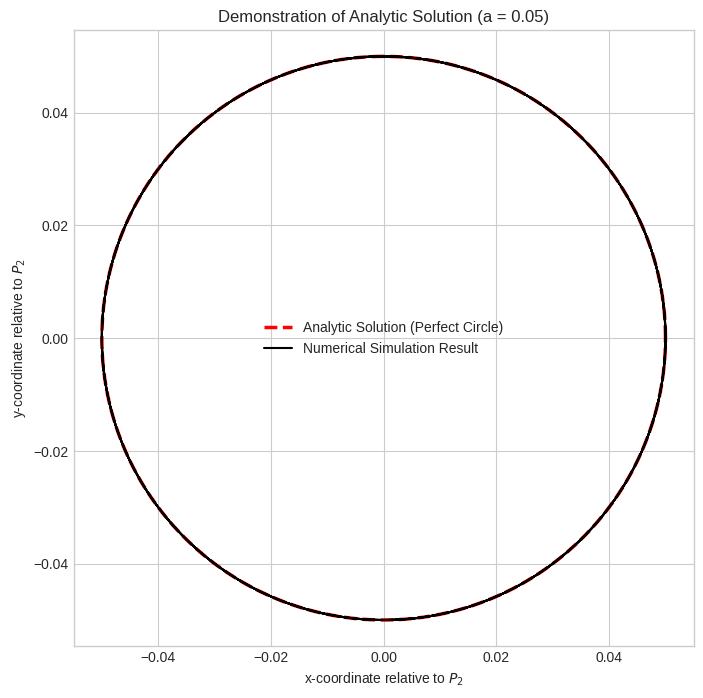
\includegraphics[width=1\linewidth]{images/circular_orbit.png}
    \caption{Comparison of the analytic solution with the numerical solution.}
\end{figure}

Returning back to the original problem but still taking equal masses \(\mu = \frac{1}{2}\), we shall take initial conditions \((x_0, y_0) = (0.2, 0)\) with initial velocities \((\dot{x}_0, \dot{y}_0) = (0, v_0)\) with \(v_0 \in \{-0.50, -1.00, -1.04, -1.18, -1.25, -1.50\}\) and we integrate on the time interval \(t \in [0, 15]\). We will plot the trajectories, the allowed region based upon the constant \(J\) and the masses involved. To ensure accuracy, we will also plot the variation of the Jacobi quantity.

\begin{figure}
    \centering
    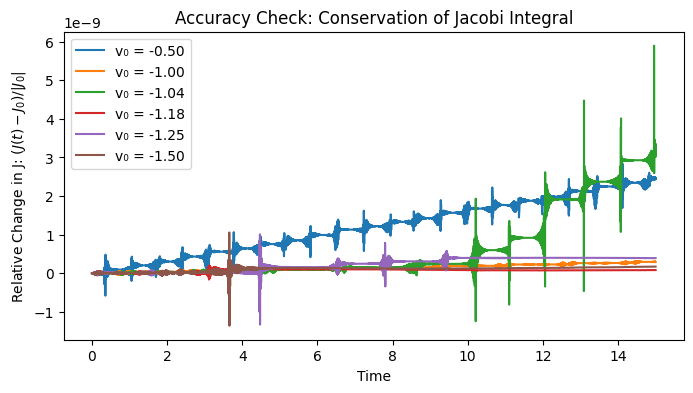
\includegraphics[width=1\linewidth]{images/spacetravel_accuracy.png}
    \caption{Variation of the relative change of the Jacobi integral over time.}
\end{figure}

We first note that the accuracy will decrease over time, yet still remains below \(10^{-8}\) for all tested cases. As the spacecraft has a close encounter with a massive body, the acceleration due to gravitational force is very high and changes direction rapidly, which leads to loss of accuracy, seem in \(v_0 = -1.25\). Furthermore, with each completed orbit, the systematic errors accumulate as seen in the case \(v_0 = 0.5\). Lastly, the case of \(v_0 = -1.04\) seems to indicate some sort of chaotic behaviour. To analyse in more detail, we will need to plot the trajectories.

\begin{figure}
    \centering
    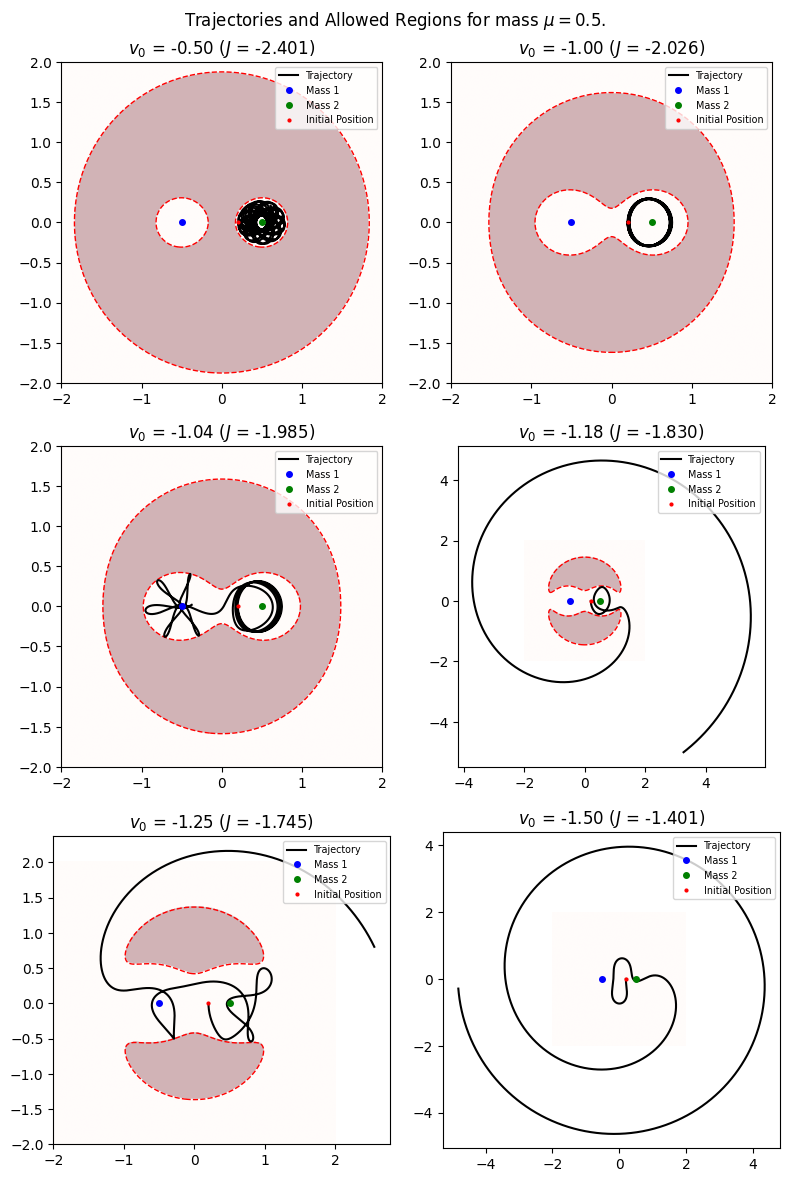
\includegraphics[width=0.95\linewidth]{images/spacetravel.png}
    \caption{Trajectories with the allowed region \(\Omega(x, y) < J\) for \(\mu = 0\) and different initial \(y\)-velocities.}
\end{figure}

Let us consider each trajectory in turn:
\begin{itemize}
    \item \(v_0 = -0.50\), the spacecraft is tightly bound to mass \(P_2\) and executes a large number of orbits in the given time interval in a dense, regular pattern. This corresponds to a large accumulation of errors causing the total energy to drift systematically but without any oscillation as there are no sudden close encounters. The spacecraft is trapped in the allowed region around \(P_2\).
    \item \(v_0 = -1.00\), this results in a simple, nearly circular orbit around mass \(P_2\) with a smooth, predictable path. With no rapid changes in acceleration, this results in a highly accurate solution. The allowed region is now connected, but while the spacecraft has enough energy to start stably orbiting \(P_2\), it does not leave the region around \(P_2\).
    \item \(v_0 = -1.04\), is the most dramatic case. The spacecraft start at \(P_2\) and is flung over to \(P_1\) where it has multiple close encounters with \(P_1\). Consequently, there is an enormous change in gravitation force, hence acceleration, causing large errors that also accumulate. Here, the spacecraft passes through the 'neck' of the allowed region.
    \item \(v_0 = -1.18\), is a simple escape trajectory. The spacecraft makes one loop about \(P_2\) and then moves away from the two mass system, with acceleration decreasing over time. In this case, the problem becomes simpler for the solver, so the accuracy is very good in this case. The neck of the allowed region has now opened up, which the spacecraft takes advantage of to enter the outer region.
    \item \(v_0 =-1.25\), is a more complicated escape trajectory where the spacecraft spends a bit more time moving between the two masses before eventually leaving. This impacts the accuracy only temporarily, demonstrated by the spike in the graph corresponding to the close encounters with the masses. The inner region has expanded, so the spacecraft spends more time performing dramatic movements.
    \item \(v_0 = -1.50\), has a completely free allowed region. The spacecraft quickly leaves the locality of the two masses and starts slowly orbiting the combined system from a large distance away. In terms of accuracy, most of the error contribution is at the beginning and there are no close encounters later on, so the accuracy remains low. There are no forbidden areas, so the spacecraft moves freely outwards.
\end{itemize}

The allowed region is a guideline to the possibility of the trajectory but not necessarily the actuality as demonstrated by the cases \(v_0 = -1.00\) and \(v_0 = -1.25\). It provides an absolute boundary for which the spacecraft can never enter. On this boundary, the potential \(\Omega\) is equal to the Jacobi \(J\), so the kinetic energy, hence velocity of the spacecraft vanishes. A trajectory approaching the boundary must slow down, arrive at the boundary with zero velocity and finally reverse its direction and move away from the boundary. Graphically, as seem in the \(v_0 = -1.04\) and \(v_0 = -1.18\) cases, the trajectory touches the boundary at a right angle and forms a sharp cusp.

At first glance, the most suitable initial \(y\)-velocity for travelling from \(P_1\) to \(P_2\) is \(v_0 = -1.04\). This is the minimal kinetic energy which allows for the transfer since any lower energy results in entrapment and a higher energy is inefficient. However, the resulting trajectory may be chaotic, so in reality, it may be more prudent to choose a higher initial energy/velocity such as \(v_0 = -1.25\) to avoid sensitivity to small perturbations and to obtain a more stable transfer.

\section{Lagrange Points}

An equilibrium point occurs when the effective forces are zero, allowing an object to remain stationary. In particular, this will occur at points where the gradient of the potential vanishes \(\nabla \Omega(x,y) =0\). On a contour plot, these critical points can occur as local saddles, minima or maxima. In general, there are give equilibrium points. Two of them create equilateral triangles with \(P_1\) and \(P_2\) as the other two vertices
\[ L_4 = \left(\mu - \frac{1}{2}, \frac{\sqrt{3}}{2}\right), \quad L_5 = \left(\mu - \frac{1}{2}, -\frac{\sqrt{3}}{2}\right). \]
The other three equilibrium points lie on the \(x\)-axis. These equilibrium points cannot be computed analytically, as the resulting equation coming from setting \(\nabla \Omega = 0\) with \(y = 0\) is a quintic. We find these points numerically, assuming that \(L_1\) occurs left of \(P_1\), \(L_2\) occurs right of \(P_2\) and finally \(L_3\) lies between the two masses. This is achieved with the below Python function. We shall then plot contour maps for \(\mu \in \{0.50, 0.30, 0.10\}\) with their corresponding equilibrium points.

\begin{minted}[autogobble, linenos]{python}
    from scipy.optimize import root_scalar
    def find_lagrange_points(mu):
        obj = lambda x, mu: calculate_Omega_and_derivatives(x, 0, mu)[1]
        eps = 1e-9 #small epsilon
        l1 = root_scalar(obj, args=(mu,), bracket=(mu-2, mu-1-eps))
        l2 = root_scalar(obj, args=(mu,), bracket=(mu-1+eps, mu+2))
        l3 = root_scalar(obj, args=(mu,), bracket=(mu-1+eps, mu-eps))
        points = [(l1.root, 0), (l2.root, 0), (l3.root, 0), 
            (mu - 0.5, np.sqrt(3) / 2), (mu - 0.5, -np.sqrt(3) / 2)]
        return points
\end{minted}

\begin{figure}
    \centering
    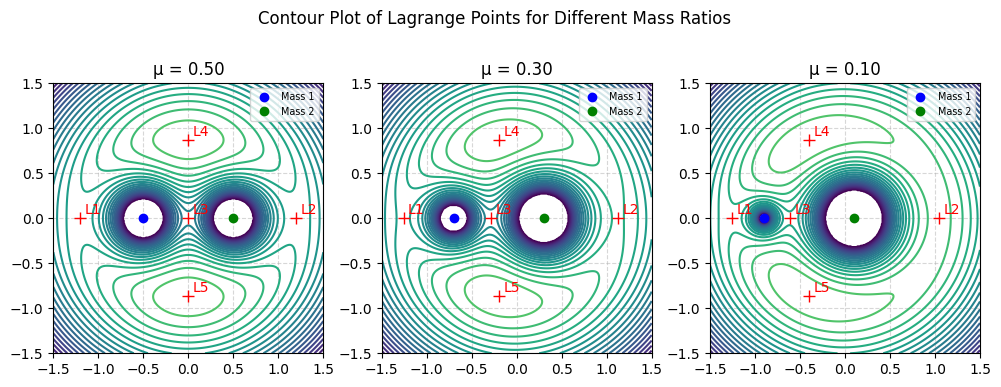
\includegraphics[width=1\linewidth]{images/lagrange_contour.png}
    \caption{Contour maps of Lagrange points.}
\end{figure}

We claim that the collinear points \(L_1, L_2, L_3\) are unstable. This can intuitively be seen from the contour plots, where the contour lines are dense around \(L_1, L_2, L_3\) and there seems to be a saddle point at this points. The stability of the equilateral points \(L_4, L_5\) depends on the mass parameter \(\mu\). 

To confirm this for the collinear equilibrium points, we perform a linearised stability analysis. Consider a small displacement \((\xi, \eta)\) from an equilibrium point \((x^*, y^*)\) so that
\[ x(t) = x^* + \xi(t), \quad y(t) = y^* + \eta(t). \]
The linearised equations of motion are

\begin{eqnarray*}
    \ddot\xi - 2\dot\eta & = & -\sder[\Omega]{xx}(x^*, y^*)\xi - \sder[\Omega]{xy}(x^*, y^*)\eta, \\
    \ddot\eta + 2\dot\xi & = & -\sder[\Omega]{yx}(x^*, y^*)\xi - \sder[\Omega]{yy}(x^*, y^*)\eta, 
\end{eqnarray*}

where the second partial derivatives are evaluated at the equilibrium point. Since the \(x\)-axis is a line of symmetry for the potential, the cross derivative term vanishes on the \(x\)-axis. Thus, the equations simplify to

\begin{eqnarray*}
    \ddot\xi - 2\dot\eta & = & -\Omega_{xx}(x^*, y^*)\xi, \\
    \ddot\eta + 2\dot\xi & = & -\Omega_{yy}(x^*, y^*)\eta.
\end{eqnarray*}

The characteristic equation for the eigenvalues of this system is given by
\[ \lambda^4 + (4 - \Omega_{xx} - \Omega_{yy})\lambda^2 + (\Omega_{xx}\Omega{yy}) = 0. \]
Let \(z = \lambda^2\) so that
\[ z^2 + (4 - \Omega_{xx} - \Omega_{yy})z + (\Omega_{xx}\Omega{yy}) = 0. \]
Contour analysis shows that \(\Omega_{xx} < 0\) as if we start at \(L_1,L_2,L_3\) and move away in the \(x\)-direction, then we are moving downhill on the potential surface. Conversely, \(\Omega_{yy} > 0\) since here we move uphill on the potential surface as the masses are positioned at the \(x\)-axis. Therefore, the product in the last term is guaranteed to be negative. This ensures the roots are real since the discriminant satisfies
\[ \Delta = (4 - \Omega_{xx} - \Omega_{yy})^2 - 4\Omega_{xx}\Omega_{yy} > 0, \]
and the roots have opposite signs, as the product of the roots is negative. In particular, the existence of a a positive root leads to instability.

For the equilateral equilibrium points, we shall investigate the behaviour of trajectories nearby and plot the distance from the equilibrium point over time.

\begin{figure}
    \centering
    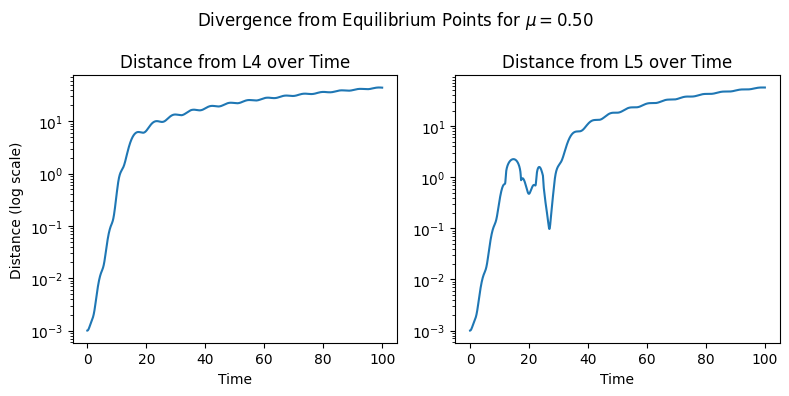
\includegraphics[width = 1\linewidth]{images/distance_0.5.png}
    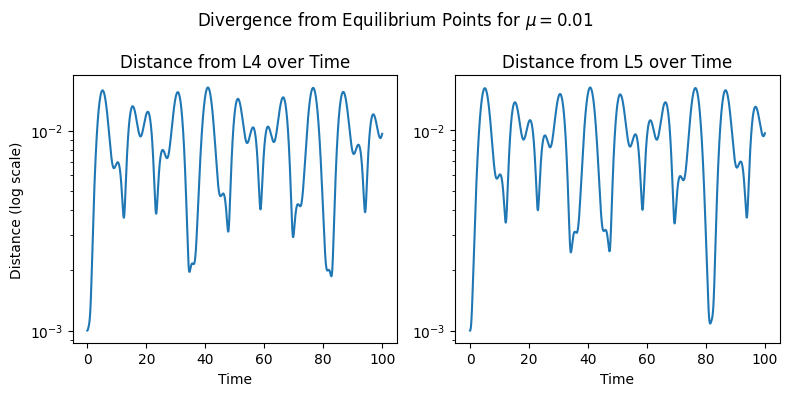
\includegraphics[width = 1\linewidth]{images/distance_0.01.png}
    \caption{Stability for small \(\mu\), instability for large \(\mu\).}
\end{figure}

From the figure, we see that the equilateral equilibriums flip from stable to unstable as we decrease \(\mu\) from \(0.5\) to \(0.01\), (and by symmetry increasing \(\mu\) also flips stability). It turns out that explicit computation of the potential and its derivatives leads to a bifurcation point at \(\mu \approx 0.0385\) which is known as Routh's mass ratio. We focus on the Lagrange point \(L_4\) since the analysis is the same for \(L_5\) by symmetry.

We return to the linearised equations of motion, where the cross derivatives now do not vanish, The characteristic equation is now
\[ z^2 + (4 - \Omega_{xx} - \Omega_{yy})z + (\Omega_{xx}\Omega{yy} - \Omega^2_{xy}) = 0, \]
the condition for stability is that both roots are real and negative. This leads to two conditions
\begin{enumerate}
    \item The discriminant must be positive
    \[ \Delta = (4 - \Omega_{xx} - \Omega_{yy})^2 - 4(\Omega_{xx}\Omega_{yy} - \Omega^2_{xy}) > 0, \]
    \item The constant term must be positive
    \[ C = \Omega_{xx}\Omega_{yy} - \Omega^2_{xy} > 0. \]
\end{enumerate}
By direct computation since we know the coordinates of \(L_4\), both \(\Omega_{xx}\) and \(\Omega_{yy}\) are negative so their product is positive and also \(\Omega^2_{xy}\) is positive. Explicitly,
\[ \Omega_{xx} = \frac{-3}{4}, \quad \Omega_{yy} = \frac{-9}{4}, \quad \Omega_{xy} = \pm \frac{3(1-2\mu)\sqrt{3}}{4}. \]
Substituting into \(C\) yields
\[ C = \frac{27\mu(1 - \mu)}{4} \]
which is always positive since \(\mu \in (0,1)\). Stability now hinges on the determinant; once again, substituting leads to the condition
\[ \Delta = 1 - 27\mu(1-\mu) > 0. \]
This is true if and only if 
\[ \mu \notin \left[\frac{9-\sqrt{69}}{18}, \frac{9+\sqrt{69}}{18}\right], \]
which is approximately \(\mu < 0.0385\) or \(\mu > 0.9615\), as required.

\begin{figure}
    \centering
    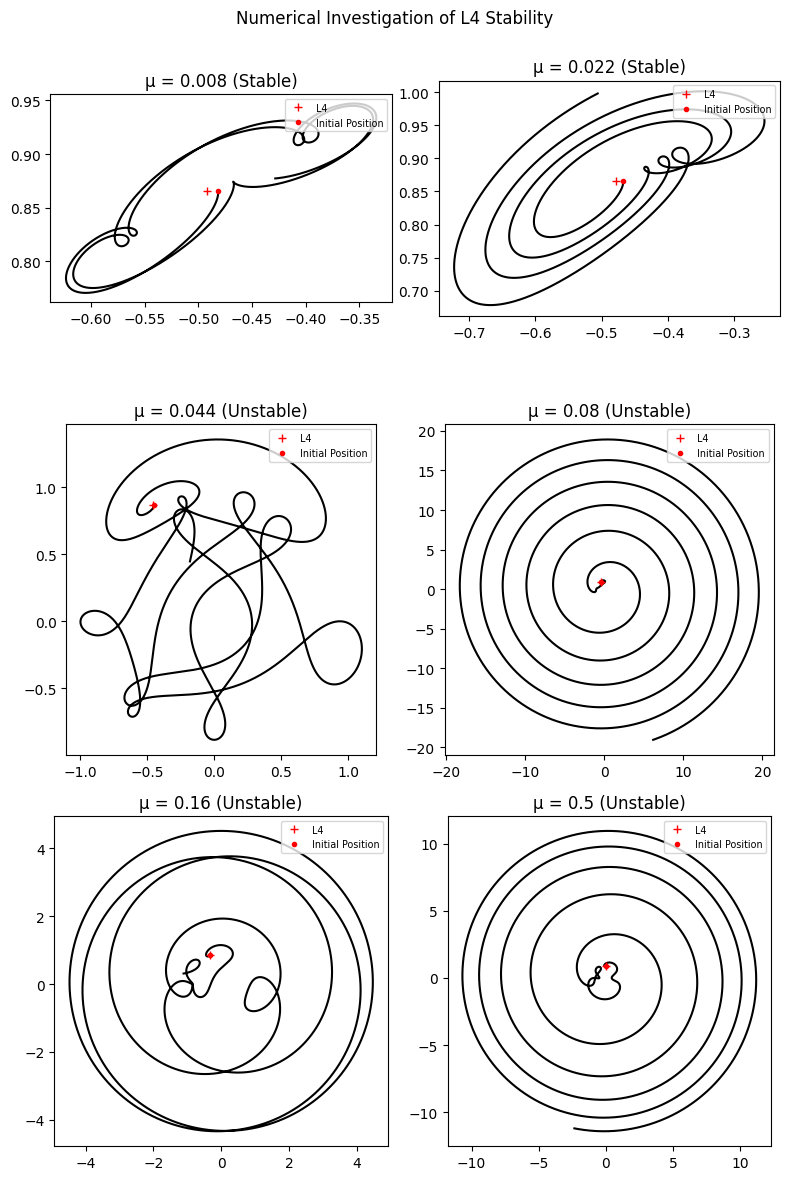
\includegraphics[width=1\linewidth]{images/l4stability.png}
    \caption{Trajectories are stable below the Routh mass ratio but unstable above.}
\end{figure}

In the small stable cases, the spacecraft does not simply return to \(L_4\), but rather the combination of gravitational and Coriolis forces compel the trajectory to  be a stable periodic orbit around \(L_4\). This is a superposition of a long-period oscillation with a short-period looping motion. In the unstable case, the discriminant is negative, giving complex conjugate roots with positive real part, corresponding to exponential growth.

For the Sun-Jupiter system, \(\mu = 9.54 \cdot 10^{-4}\) and the Trojans are a group of asteroids which can be observed at the equilateral Lagrange point. Analogously for the Earth-Moon system, there is evidence for the existence of Kordylewski clouds are the equilateral Lagrange points. Both these scenarios are consistent with our analysis, since \(\mu\) is less than Routh's mass ratio. Lastly, the James Webb telescope is in a stable orbit in the \(L_2\) point of the Sun-Earth system.

\section{Schr\"odinger's Equation}

Consider a particle of mass \(m\) and energy \(\epsilon\) in a real one-dimensional potential \(v(x)\). The Schr\"odinger time-independent wave equation is
\[ \left[-\frac{\hbar}{2m}\frac{d^2}{dx^2} + v(x)\right]\psi(x) = \epsilon\psi(x), \]
where \(2\pi\hbar\) is Planck's constant. The state of the system is represented by a complex time-dependent wave function \(\psi(x)e^{-i\epsilon t/\hbar}\).

Let \(\epsilon_1\) be the unit of energy so that \(E = \epsilon/\epsilon_1\) is the dimensionless potential energy. Define a dimensionless coordinate \(X = x\sqrt{2m\epsilon_1}/\hbar\). Then the equation simplifies as
\[ \left[-\frac{d^2}{dX^2} + V(X)\right]Y(X) = EY(X) \]
where \(V(X) = v(x)/\epsilon_1\) is the dimensionless potential energy and \(Y(X) = \psi(x)\) is the stationary wave function. 

In a bound state, in which the particle is localised near \(X = 0\), we have \(Y(X) \to 0\) as \(|X| \to \infty\) sufficiently fast such that the wave function is normalisable
\[ \int_{-\infty}^{\infty} |Y(X)|^2 \,dX < \infty. \]
Furthermore, the real and imaginary parts of \(Y\) decay monotonically for sufficiently large positive or negative \(X\). Such solutions to the Schr\"odinger equation only exist for certain values of \(E\), which are the eigenvalues of the equation.

\section{Quantum Harmonic Oscillator}

Consider the harmonic oscillator potential
\[ V(X) = X^2. \]
The general solution for the Schr\"odinger equation is given by
\[ Y(X) = [c_ef_e(X) + c_of_o(X)]\exp(-X^2/2), \]
where \(f_e\) is an even function and \(f_o\) is an odd function. The constants \(c_e\) and \(c_0\) depend on the initial conditions \(Y(0)\) and \(Y'(0)\). We assume the properties
\begin{itemize}
    \item Normalisable solutions exist if and only if \(E\) is an odd positive integer, otherwise all solutions diverge as \(|X| \to \infty\).
    \item If \((E-1)/2\) is an even integer then any normalisable solution must be even \(c_o = 0\). Similarly, if \((E-1)/2\) is an odd integer, then any normalisable solution must be odd \(c_e = 0\).
    \item The functions \(f_e\) and \(f_o\) that appear in normalisation solutions are Hermite polynomials, e.g. for \(E = 1, 3, 5\) we have \ \(1, X, 1-2X^2\). In general
    \[ f_e(X) = \sum_{n=0}^\infty a_n X^{2n}, \quad f_0(X) = \sum_{n=0}^\infty b_n X^{2n+1}, \]
    where \(a_0 = 1\), \(b_0 = 1\) and we have the recurrence relations
    \[ a_{n+1} = \frac{4n+1-E}{(2n+2)(2n+1)}a_n, \quad b_{n+1} = \frac{4n+3-E}{(2n+3)(2n+2)}b_n. \]
\end{itemize}

Let us first restrict to the odd solutions by taking the initial conditions \(Y(0) = 0\) and \(Y'(0) = 1\). We shall first convert our second order ODE into a system of two linear ODEs using the state vector \(S = (Y, Y')\) so that
\[ \frac{dY}{dX} = Y', \quad \frac{dY'}{dX} = (X^2- E)Y. \]
It is now straightforward to use a standard Python initial value problem solver to solve this system of ODEs for a given value of \(E\), initial values and range of integration \(X \in [0, X_{\max}]\).

\begin{minted}[autogobble, linenos]{python}
    def harmonic_oscillator(X, S, E):
        Y, Y_prime = S
        return [Y_prime, (X**2 - E) * Y]
    
    def solve_schrodinger_ode(func, E, S0, X_max, n_points, tol):
        X_eval = np.linspace(0, X_max, n_points)
        solution = solve_ivp(
            fun=lambda X, S: func(X, S, E),
            t_span=[0, X_max],
            y0=S0,
            t_eval=X_eval,
            dense_output=True,
            atol = tol,
            rtol = tol
        )
        return solution
\end{minted}

Set \(E = 2.9\) and \(X_{\max} = 5\). We confirm the accuracy of \(Y(5)\) by adjusting the tolerance value.
\begin{verbatim}[Convergence of the numerical estimates of Y(5)]
    Value of Y(5)       Tolerance (tol)
    277.6757273773642   1e-04
    278.1010417934544   1e-06
    278.10240962411814  1e-08
    278.10240915297067  1e-10
    278.10240910456747  1e-12
\end{verbatim}

This confirms that our solver is accurate up to six significant figures. Let us plot the solutions of a small perturbation each side of the energy \(E = 2.9995\) and \(E = 3.0005\).

\begin{figure}
    \centering
    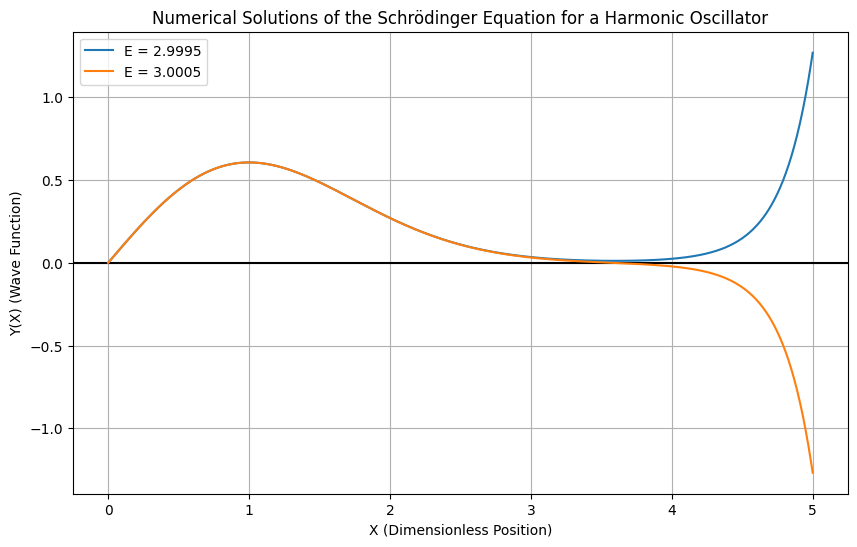
\includegraphics[width=1\linewidth]{images/harmonic_1.png}
    \caption{Perturbation about a bound state.}
\end{figure}

This agrees with the theoretical analysis of bound states, for they are the only solutions which are normalisable, below the eigenvalue our solution diverges to infinity whereas above the eigenvalue our solution diverges to negative infinity. Furthermore, by uniqueness of solution to initial values problems, trajectories cannot cross which agrees with the opposite divergence property.

We can argue as follows. The equation
\[ \frac{d^2Y}{dX^2} = (X^2 - E)Y(X) \]
tells us that the curvature of the wave function is determined by the product of \(X^2 - E\) with the wave function itself. Beyond the region \(X > 5\), we see that \(X^2 - E\) is positive and tends to infinity as \(X \to \infty\). Therefore, we see that the sign of the curvature is the same as the sign of the function in this region. Consequently, we see that for \(E = 2.9995\), since \(Y(5) > 0\), the function becomes more and more convex, ultimately diverging to infinity. The exact opposite holds for \(E = 3.0005\). In summary, once the solution enters the region where \(X^2 > E\), it chooses a direction and the curvature pushes accelerates it in this direction, ensuring monotonic divergence.

\begin{figure}
    \centering
    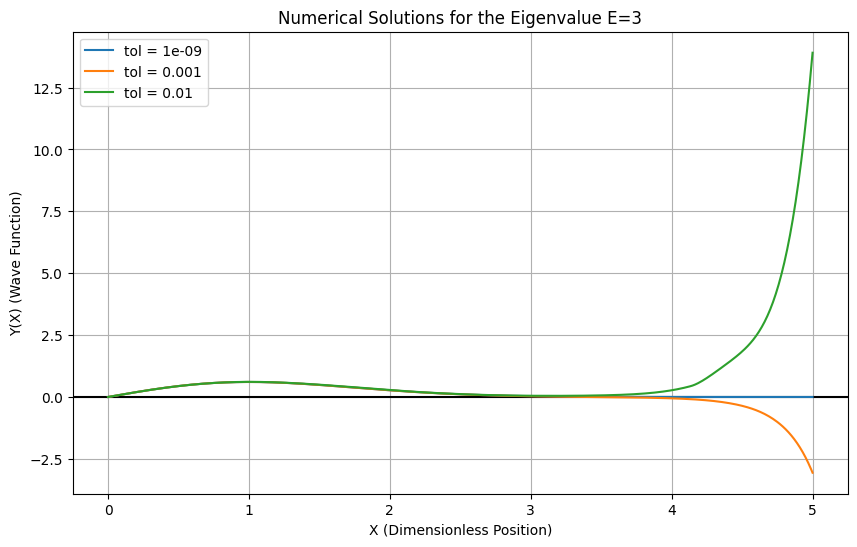
\includegraphics[width=1\linewidth]{images/harmonic_2.png}
    \caption{Numerical instability of the eigenvalue solution.}
\end{figure}

The eigenvalue \(E = 3\) provides a boundary between the negative and positive divergence where the function perfectly decays to zero as \(\exp(-X^2/2)\) since the curvature is decaying to zero. Numerically, the solution will not decay to zero for large \(X\). Instead, it follows a decaying solution for some finite time, but eventually will diverge exponentially owing to the precision errors which 'contaminate' the perfect eigenvalue solution by introducing a divergent superposition which eventually blows up. A more accurate solver will follow the decaying solution for longer.

\section{Nearby-Square Potential Well}

We now turn to the potential defined by
\[ V(X) = -\frac{\Delta V}{1+X^4} \]
where \(\Delta V > 0\) is a constant. As before, odd solutions come from taking \(Y(0) = 0\) and \(Y'(0) = 1\) whereas even solutions come from taking \(Y(0) = 1\) and \(Y'(0) = 0\). 

There is no loss of generality to restricting to either odd or even solutions since the potential is an even function. Since the kinetic energy \(\frac{d^2Y}{dX^2}\) is also an even function, this means that the entire Hamiltonian operator is even. Consequently, if \(Y(X)\) is a solution to the Schr\"odinger equation, then \(Y(-X)\) is also necessarily a solution. There can only be one linearly independent solution for each bound sate by uniqueness so \(Y(-X) = cY(X)\) for some \(c \in \mathbf{R}\). But
\[ Y(X) = Y(-(-X)) = cY(-X) = c^2Y(X), \]
which implies that \(c = \pm 1\). The solution is (purely) even if \(c = 1\) and odd if \(c = -1\).

The shallow potential is when \(\Delta V = 1\). It turns out there is exactly one bound state which we verify by checking various energies from \(-1\) to \(0\) for both odd and even solutions. 

\begin{minted}[autogobble, linenos]{python}
    def shallow_well(X, S, E):
        Y, Y_prime = S
        return [Y_prime, (-1 / (1 + X**4) - E) * Y]
\end{minted}

We see that only one bound state exists in the interval \((-1,0)\) and that it is an even function. Trajectories cannot cross by uniqueness, so we can be sure that we only have one bound state that is an even function and no bound states that are odd functions.

\begin{figure}
    \centering
    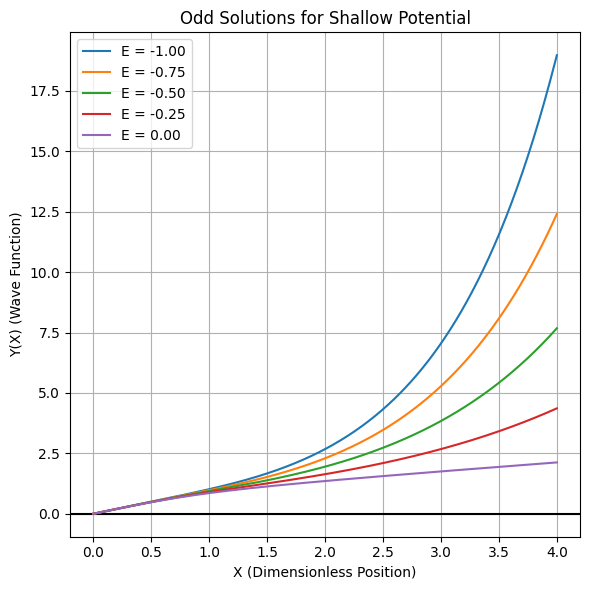
\includegraphics[width=0.49\linewidth]{images/old_shallow.png}
    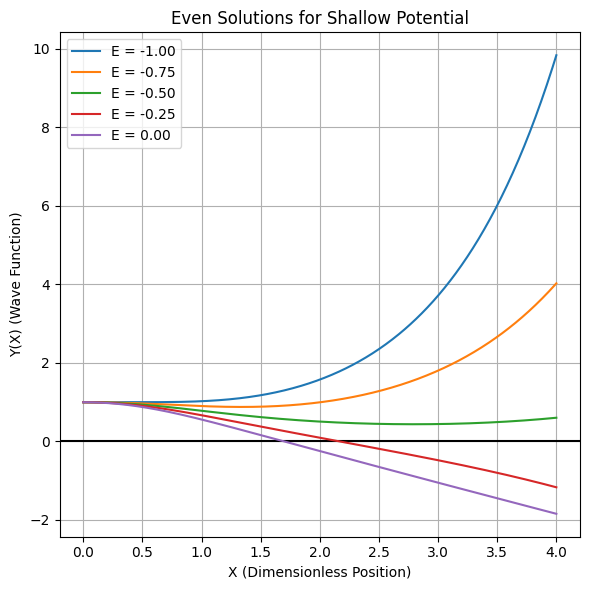
\includegraphics[width=0.49\linewidth]{images/even_shallow.png}
    \caption{One even bound state exists.}
\end{figure}

 We can exclude any energies \(E > 0\) as the potential \(V(X) \to 0\) as \(|X| \to \infty\) and in the limit the Schr\"odinger equation becomes
\[ \frac{d^2Y}{dX^2} \approx -E Y, \]
which is a simple harmonic oscillator. Solutions oscillate indefinitely so do not decay. These represent a scattering state of a free, unbounded particle that is not trapped inside a well potential. We can also rule out any bound states with energy \(E < \Delta E\). The minimum value of the potential occurs at \(X = 0\) where \(V_{\min} = -\Delta V\). Here, the total energy \(E\) is less than the minimum potential energy so \(V(X) - E > 0\). By the same analysis of the harmonic oscillator potential, the sign of the curvature matches the sign of the function leading to monotonic divergence, hence a bound state is impossible.

Using interval bisection, we can attempt to find the negative eigenvalue up to three significant figures.

\begin{minted}[autogobble, linenos]{python}
    def find_eigenvalue_bisection(func, S0, X_max, E_left, E_right, tol=1e-6):
        E_low, E_high = E_left, E_right
        sign_at_low = np.sign(getY_at_Xmax(func, E_low, S0, X_max))
        sign_at_high = np.sign(getY_at_Xmax(func, E_high, S0, X_max))
        if sign_at_low == sign_at_high:
            raise ValueError("Cannot apply bisection.")
        while (E_high - E_low) > tol:
            E_mid = (E_low + E_high) / 2
            y_mid_sign = np.sign(getY_at_Xmax(func, E_mid, S0, X_max))
            if y_mid_sign == sign_at_low:
                E_low = E_mid
            else:
                E_high = E_mid
        return E_low, E_high
\end{minted}

We shall test the final value for \(X_{\max} = 8\) using the initial values for an even solution \(Y(0) = 1\) and \(Y'(0) = 0\). The potential at \(X = 8\) is given by \(V(8) = -0.00024\) which is close to zero and ensures that asymptotic behaviour is already established to the appropriate tolerance.

\begin{figure}
    \centering
    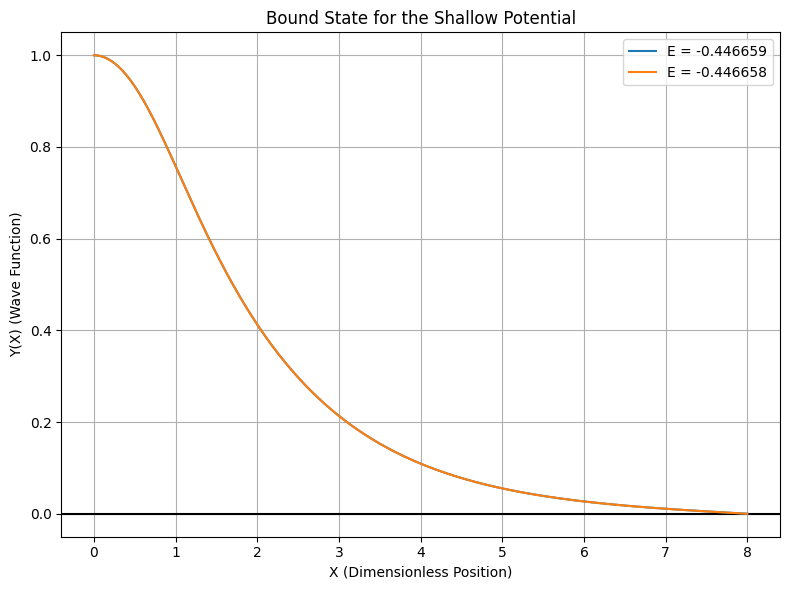
\includegraphics[width=1\linewidth]{images/bound_shallow.png}
    \caption{Final bracketing interval: \([-0.446659, -0.446658]\). Estimated eigenvalue: \(-0.446659\).}
\end{figure}

Looking at the asymptotic behaviour of the system, the potential approaches zero so the equation simplifies to
\[ \frac{d^2Y}{dX^2} \approx |E| Y. \]
As a second order linear ODE, this has a general solution of the superposition of a growing exponential and a decaying exponential with exponent \(\sqrt{|E|}\). For the solution to be a bound state, the normalisation property implies that the coefficient of the growing exponential is zero. We have observed that for \(E = -1\) the coefficient is positive, whereas for \(E = 0\) the coefficient is negative. 

Crucially, a property of solutions to linear ODEs is that these coefficients are continuous functions of the parameter \(E\). Therefore, we may apply the intermediate value problem to obtain an energy in the interval \((-1, 0)\) for which the coefficient vanishes. This corresponds precisely to a bound state.

For larger potentials \(\Delta V > 1\), there tend to be more bound states. We assume two theoretical results.

\begin{enumerate}
    \item Consider a square potential well of width \(2L\):
    \[ V_{\mathrm{square}}(X) = -\Delta V, \mbox{ if } |X| < L, \]
    and zero otherwise. This potential has precisely \(N\) bound states if 
    \[ \frac{2L}{\pi}\sqrt{\Delta V} \in (N-1, N]. \]
    Bound states for the square potential and the strong potential well turn out to be qualitatively similar, but one must choose \(L\) appropriately. For example, one might estimate the ‘width’ of the strong potential well as
    \[ L = \left(\frac{\int_0^\infty X^2V(X)\,dX}{\int_0^\infty V(X)\,dX}\right)^{1/2} = 1. \]
    \item The WKB approximation can be used to analyse where \(\Delta V\) is very large. Specifically, as \(\Delta V \to \infty\), then the bound state energies asymptote to \(\widetilde{E}_n = -\Delta V/(1+X^4_n)\) for \(n = 0, 1, \dots, N-1\), where \(N\) is the number of bound states and \(X_n\) is determined by
    \[ \int_{-X_n}^{X_n} \sqrt{\widetilde{E}_n - V(X)}\,dX =\left(n+\frac{1}{2}\right)\pi. \]
    Also, \(N\) is determined asymptotically by the condition that
    \[ \frac{2\widetilde{L}}{\pi}\sqrt{\Delta V} \in (N - 1/2, N + 1/2], \]
    where
    \[ \widetilde{L} = \frac{1}{2}\int_{-\infty}^\infty \sqrt{\frac{-V(X)}{\Delta V}}\,dX = \int_0^\infty \frac{dX}{\sqrt{1+X^4}} \approx 1.85. \]
\end{enumerate}

Take \(\Delta V = 36\). Then 
\[ \frac{2\widetilde{L}}{\pi}\sqrt{\Delta V} = \frac{22.2}{\pi} \approx 7.066 \in [N-1/2, N+1/2] \]
which is satisfied if and only if \(N = 7\). Therefore, we would expect \(7\) bound states which are ordered by their energy \(E_0 < \cdots < E_6\) with alternating parity.

\begin{minted}[autogobble, linenos]{python}
    def deep_well(X, S, E):
        Y, Y_prime = S
        return [Y_prime, (-36 / (1 + X**4) - E) * Y]
\end{minted}

We take a high-precision tolerance of \(10^{-12}\) to ensure good accuracy throughout. First of all, we implement a quadrature solver to obtain the WKB approximation of \(\widetilde{E}_n\) in terms of the turning points \(X_n\).

\begin{minted}[autogobble, linenos]{python}
    from scipy.integrate import quad
    from scipy.optimize import root_scalar
    def calculate_wkb_energies(num_states):
        wkb_results = []
        def wkb_integrand(X, Xn):
            return 6 * np.sqrt(1/(1 + X**4) - 1/(1 + Xn**4))
        for n in range(num_states):
            def wkb_equation_to_solve(Xn):
                int_val, _ = quad(wkb_integrand, -Xn, Xn, args=(Xn,))
                return int_val - (n + 0.5) * np.pi
            sol = root_scalar(wkb_equation_to_solve, bracket=[0.1, 10])
            Xn_sol = sol.root
            E_wkb = -36 / (1 + Xn_sol**4)
            wkb_results.append({'n': n, 'E_wkb': E_wkb, 'Xn_wkb': Xn_sol})
        return wkb_results
\end{minted}

Using this function, we obtain the asymptotic bound states for large \(\Delta V\). We are also able to confirm that there are no more than seven states exist, given a failure in the script to find any other turning points.

\begin{verbatim}[WKB asymptotic approximations]
    n=0:    Xn = 0.5394     E_wkb = -33.1913
    n=1:    Xn = 0.8238     E_wkb = -24.6491
    n=2:    Xn = 1.0677     E_wkb = -15.6542
    n=3:    Xn = 1.3679     E_wkb = -7.9983
    n=4:    Xn = 1.8508     E_wkb = -2.8269
    n=5:    Xn = 2.9357     E_wkb = -0.4782
    n=6:    Xn = 7.8704     E_wkb = -0.0094
\end{verbatim}

We then use the following algorithm to search for an initial bracket for which we perform our bisection method. We also include two functions which check the asymptotic sign and count the number of zeros of the bound state.

\begin{minted}[autogobble, linenos]{python}
    def find_bracket(func, S0, X_max, E_min, E_max, delta_E=0.1):
        E_guess = E_min
        sign_guess = np.sign(getY_at_Xmax(func, E_guess, S0, X_max))
        E_up = E_guess + delta_E # Search up
        while E_up < E_max:
            if np.sign(getY_at_Xmax(func, E_up, S0, X_max)) != sign_guess:
                return [E_guess, E_up]
            E_up += delta_E
        E_down = E_guess - delta_E # Search down
        while E_down > E_min:
            if np.sign(getY_at_Xmax(func, E_down, S0, X_max)) != sign_guess:
                return [E_down, E_guess]
            E_down -= delta_E

    def get_asymptotic_sign(func, E, S0, X_max):
        sol = solve_ivp(fun=lambda X, S: func(X, S, E), t_span=[0, X_max], y0=S0,
                        t_eval=[X_max], rtol=1e-14, atol=1e-14)
        return np.sign(sol.y[0, -1])

    def count_zeroes(solution, parity):
        y_values = solution.y[0]
        sign_changes = np.where(np.diff(np.sign(y_values)))[0]
        return 2 * len(sign_changes) if parity == 'even' else 2 * len(sign_changes) + 1
\end{minted}

Note that we can take \(E_{\min} = -\Delta V = -36\) and \(E_{\max} = 0\) initially and then successively update the minimum to be the previous found eigenvalue. However, our \(X_{\max}\) must now be chosen carefully. For very negative eigenvalues, we should take it smaller to avoid precision blow up, whereas for eigenvalues close to zero, it must be taken larger to observe asymptotic behaviour. 

Our turning points for the WKB approximation can form the basis of a good value of \(X_{\max}\) and their corresponding energy values will form our first guess of each eigenvalue for our deep well potential. In particular, we will take five times the turning point for \(X_{\max}\) for each WKB approximation.

\begin{figure}
    \centering
    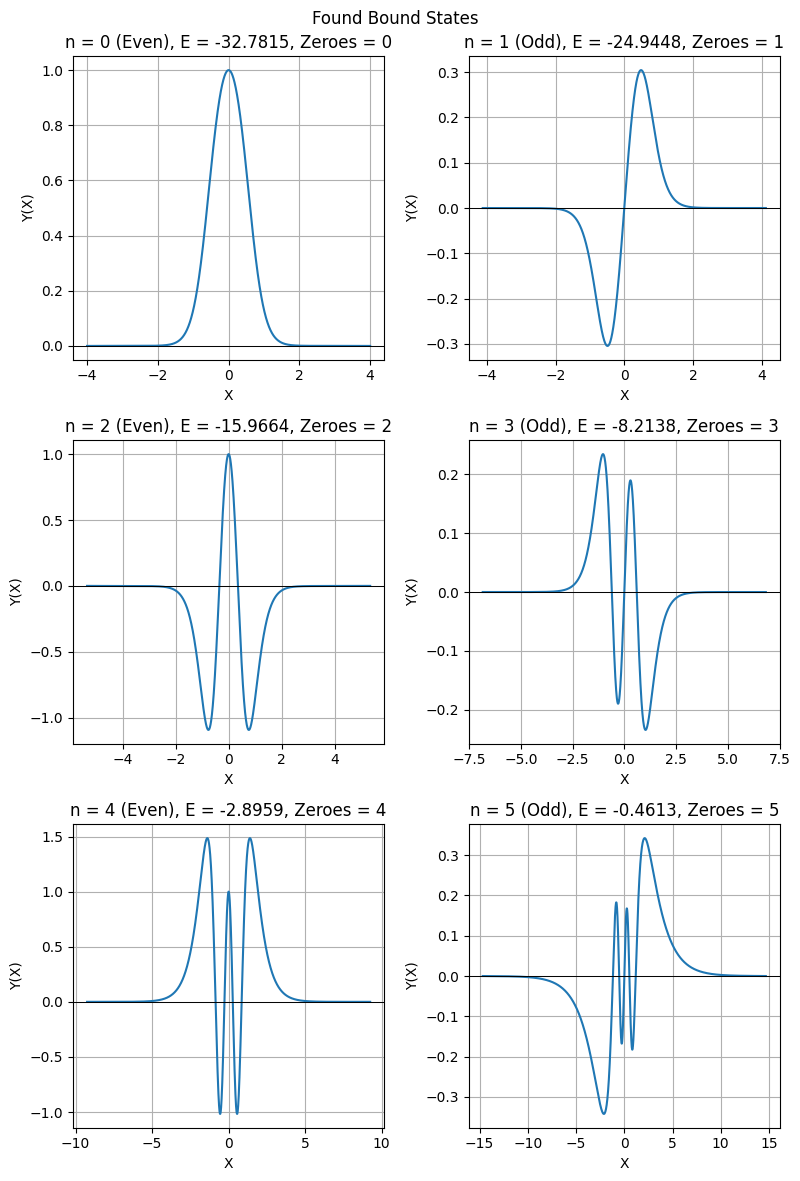
\includegraphics[width=1\linewidth]{images/bound_states.png}
    \caption{Bound states for the deep well potential.}
    \label{fig:placeholder}
\end{figure}

Our program finds the following bound states:

\begin{verbatim}
    n     Parity     Eigenvalue E_n       No. of Zeroes    
    0     Even       -32.7815             2                   
    1     Odd        -24.9448             3                   
    2     Even       -15.9664             4                   
    3     Odd        -8.2138              5                   
    4     Even       -2.8959              4                   
    5     Odd        -0.4613              9           
\end{verbatim}

We have taken many precautions to ensure sufficient accuracy.
\begin{enumerate}
    \item WKB informed guesses which are close to the desired eigenvalues.
    \item Robust bracketing in the bisection which expands the search interval until the intermediate value theorem can be applied.
    \item Adaptive integration range. This is important for precision and to avoid precision blow up for the lower energy states and ensure that we capture asymptotic behaviour for the higher energy states.
    \item High precision ODE solvers and verification of the sign of the function, which can be verified qualitatively by counting the nodes in the plots.
\end{enumerate}

The agreement between the numerical result and the WKB approximation of the square well is fairly accurate for the lower energy bound states but drifts as we go to higher energy states. It also agrees with the fact that the energy states get closer together as \(E \to 0\). Nevertheless, we only found six out of the suggested seven bound states. There could be two reasons for the discrepency. Either there are genuinely only six bound states and the WKB approximation fails due to \(\Delta V = 36\) not being large enough, or we have reached the limitation of precision of the Python ODE solver and we must use additional computation time to find the final bound state.

\end{document}
